\documentclass{article}
\usepackage{graphicx}
\usepackage{amsmath}
\usepackage{amsthm}
\usepackage{listings}
\usepackage{xcolor}
\newtheorem*{theorem*}{Theorem}

\lstset{language=python, basicstyle=\ttfamily\small, 
        keywords={read, mean, subplots, plot, set_xlabel, set_ylabel, set_title, savefig, close, copy, linspace, fft, fftshift, argmax, ifft, ifftshift},
        keywordstyle=\color{purple}, commentstyle=\color{gray}, stringstyle=\color{blue}}
\setcounter{section}{-1}

\begin{document}
    \begin{center}
		\textbf{\huge Signals Project Report}
        \\ \vspace{50pt}
        \Large Ain Shams University \\ Faculty of Engineering
        \\ \vspace{15pt}
        \textbf{Under the Supervision of}
        \\
        \textit{\Large Prof. Ahmed Othman}
        \\[1.5cm]
        \textbf{\Large Team Members}
        \\[0.5cm]
        \begin{tabular} { c  c  c }
            \textbf{Name} & \textbf{Code} & \textbf{Section} \\[5pt]
            \hline \\[-10pt]
            \textit{\Large Mohamad Ibrahim} & \textit{\Large 2401339} & \textit{\Large 7} \\
            \textit{\Large Mohammad Abduljalil Mohammad Al Saeid} & \textit{\Large 2400877} & \textit{\Large 7} \\
            \textit{\Large Mena Elia} & \textit{\Large 24*****} & \textit{\Large 7} \\
            \textit{\Large Mohammad Hany} & \textit{\Large 2400615} & \textit{\Large 7} \\
            \textit{\Large Moaz Wael} & \textit{\Large 240****} & \textit{\Large 7} \\
            \textit{\Large Moaaz Mostafa Ibrahim} & \textit{\Large 2400862} & \textit{\Large 7} \\
        \end{tabular}
	\end{center}
\clearpage

\section{Tools Used}
To be able to implement this project in python multiple libraries must be imported for audio file reading/writing, FFT, array manipulation, and graphing.
For audio files, \texttt{soundfile} was used. \texttt{Numpy} was used for FFT, IFFT, and array manipulation, along with \texttt{matplotlib} for plotting.

\section{Time Domain Signal}
A few lines of code can be used to extract the audio signal and plot it provided the audio file is in \texttt{.wav} format.
After reading the file, we must change the shape (dimensions) of the array to a 1D array representing a mono audio signal.

\begin{lstlisting}
x_t, f_s = sf.read('Moaaz.wav')

# Convert to mono
x_t = x_t.mean(axis=1) if x_t.ndim > 1 else x_t
# Define time domain
t = np.linspace(0, len(x_t) / f_s, num=len(x_t))
\end{lstlisting}

\noindent
We can then plot\footnote{This plotting code will be used many times throughout the report. 
We will only show it this time but any plot in the report was generated similarly.} the signal as shown in figure (\ref{fig:moaaz_signal}).

\begin{lstlisting}
time_fig, time_ax = plt.subplots()

time_ax.plot(t, x_t, color='k')
time_ax.set_xlabel('Time [s]')
time_ax.set_ylabel('Amplitude')
time_ax.set_title('Audio Signal')

time_fig.savefig('Moaaz_Signal.png')
plt.close(time_fig)
\end{lstlisting}
\clearpage

\begin{figure}[h!]
    \centering
    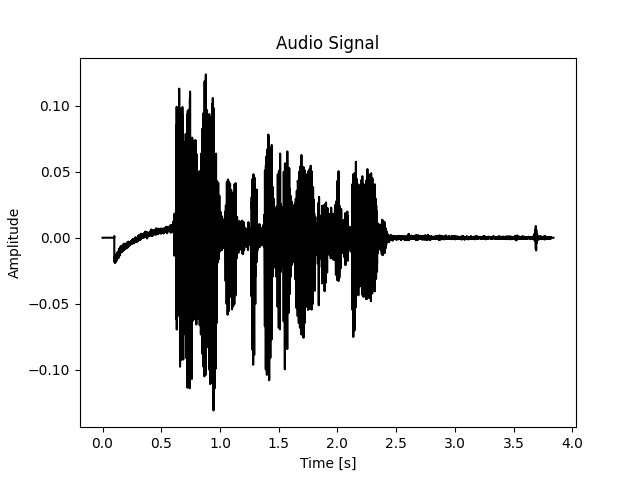
\includegraphics[width=0.75\textwidth]{Plots/Moaaz_Signal.png}
    \caption{Time Domain Signal}
    \label{fig:moaaz_signal}
\end{figure}

\noindent
Lastly, we need to calculate the energy of the signal in the time domain using \lstinline|np.sum(x_t**2)|.
\begin{equation*}
    E = \sum_{n=-\infty}^{\infty} |x(n)|^2 \approx 46.3
\end{equation*}


\section{Frequency Domain Signal}
Using \texttt{numpy}, we apply the Fourier transform to the audio signal to obtain its frequency spectrum.
Then we plot the signal in the frequency domain. 
To better examine the frequencies, we also present a zoomed-in version of the plot in figure (\ref{fig:moaaz_frequency}).

\begin{lstlisting}
import numpy.fft as FT
# FT centered around zero frequency
X_f = FT.fftshift(FT.fft(x_t)) 
# Define frequency domain
f = np.linspace(-f_s/2, f_s/2, len(X_f), endpoint=False)
\end{lstlisting}

\begin{figure}[h]
    \centering
    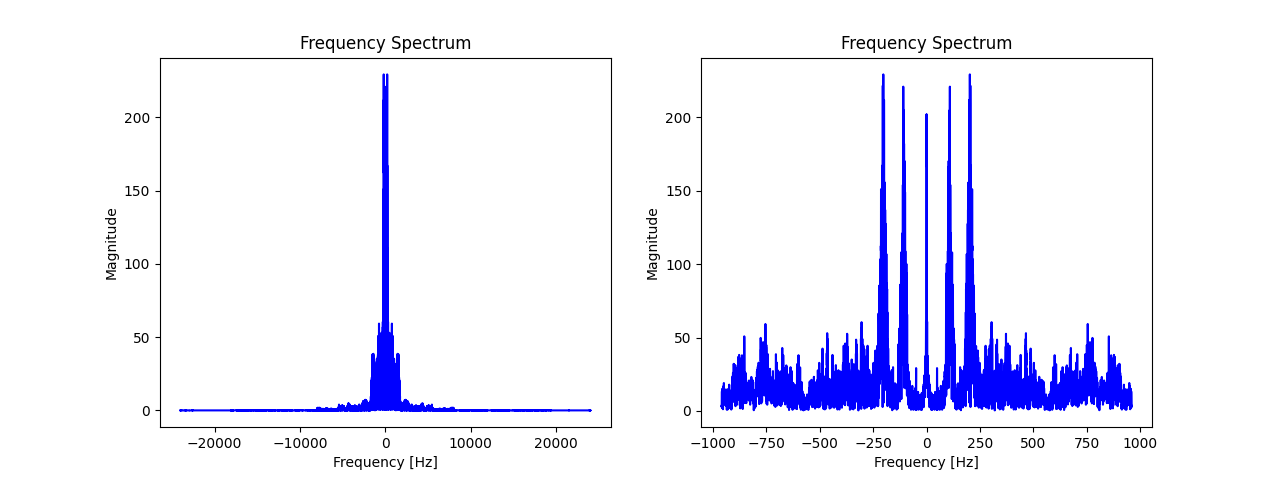
\includegraphics[width=\textwidth]{Plots/Moaaz_Frequency_Spectrum.png}
    \caption{Frequency Domain Signal}
    \label{fig:moaaz_frequency}
\end{figure}

\noindent
If we calculate the energy of the signal in the frequency domain over a single period.
\begin{equation*}
    E = \sum_{k=0}^{N-1} |X(k)|^2 \approx 8533804.3
\end{equation*}
\noindent
But Perseval's theorem says that the energy in both domains should be equal!
Now we must remember that a computer doesn't calculate CTFT, it calculates DTFT where Perseval's theorem has different statement.

\begin{theorem*}[Perseval's Theorem for DTFT]
    \begin{equation*}
        \sum_{n=-\infty}^{\infty} |x(n)|^2 = \frac{1}{2\pi} \int_{-\pi}^{\pi} |X(e^{j\omega})|^2 d\omega
    \end{equation*}
\end{theorem*}

\noindent
So if we calculate the \textit{average power} of the frequency domain signal using \lstinline|np.mean(np.abs(X_f)**2)| we can verify Perseval's theorem in this case.
\begin{equation*}
    \bar{P} = \frac{1}{N} \sum_{k=0}^{N-1} |X(k)|^2 \approx 46.3
\end{equation*}

\noindent
But to find the exact frequency with maximum contribution to the signal we can use a very useful function in \texttt{numpy} called \lstinline|argmax|.
\begin{lstlisting}
index_max = np.argmax(np.abs(X_f))
f_max = f[index_max]
\end{lstlisting}
And we find that frequency to be $\approx 202.6$ Hz.

\section{Notch Filter}
Given the Fourier transform of the signal we can implement an ideal notch filter by simply removing any desired frequency band.
We implemented this notch filter with a bandwidth of 50, 100, and 200 Hz with the shown results.

\begin{lstlisting}
bw = 50 # Notch filter bandwidth
window = bw//df
lower_bound = int(index_max - window//2)
upper_bound = int(index_max + window//2)

Notch_50Hz = X_f.copy()
Notch_50Hz[lower_bound:upper_bound] = 0
Notch_50Hz[len(X_f) - upper_bound:len(X_f) - lower_bound] = 0
\end{lstlisting}

\begin{figure}[h]
    \centering
    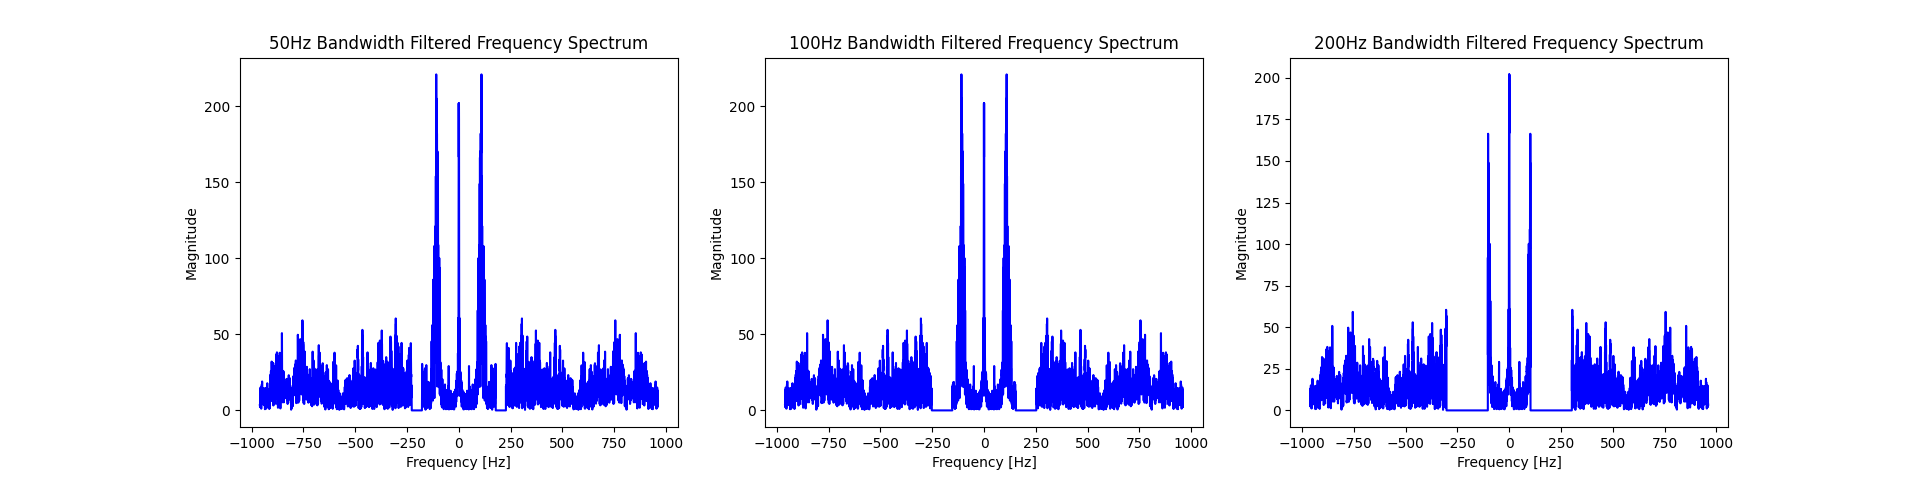
\includegraphics[width=\textwidth]{Plots/Moaaz_Frequency_Spectrum_Filtered.png}
    \caption{Frequency Spectrum after Notch Filtering}
    \label{fig:moaaz_filtered_frequency}
\end{figure}

\begin{figure}[h]
    \centering
    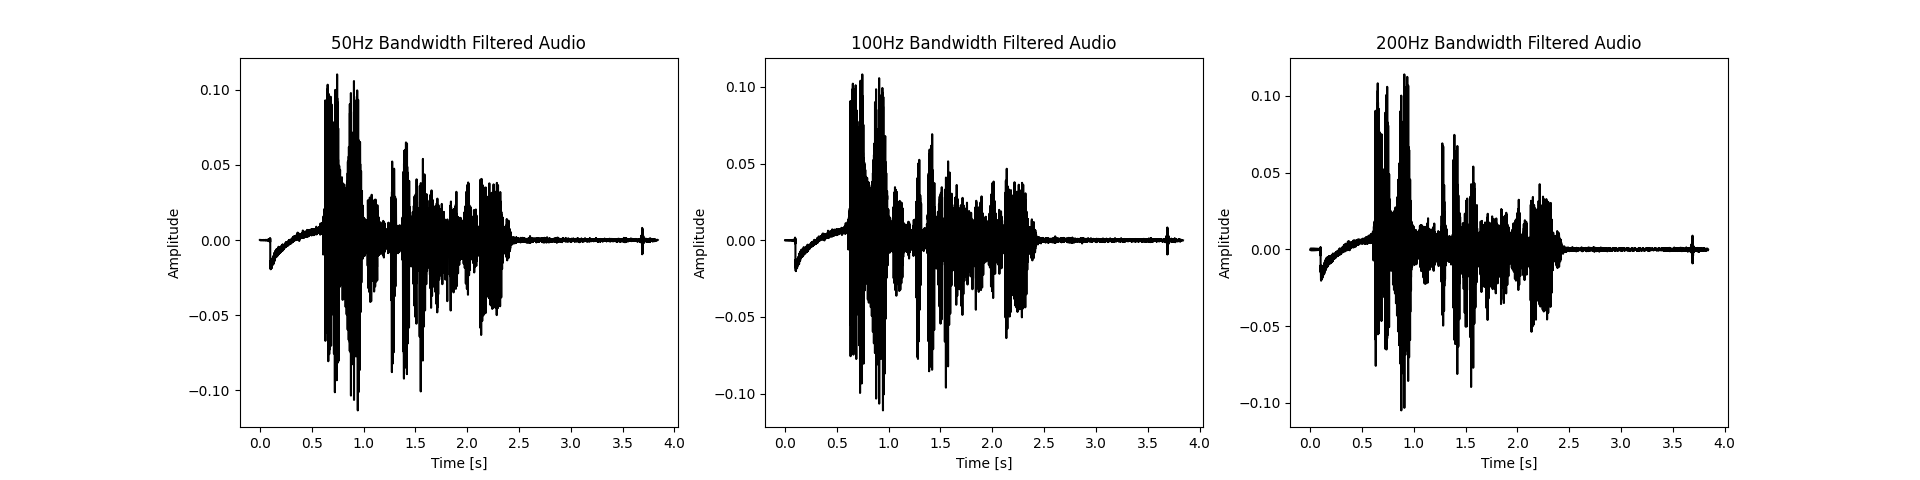
\includegraphics[width=\textwidth]{Plots/Moaaz_Time_Signal_Filtered.png}
    \caption{Time Domain Signal after Notch Filtering}
    \label{fig:moaaz_filtered_time}
\end{figure}

\end{document}